\chapter{Mathematical Tools}
\label{chapter1}

\section{An overview of Differential Geometry}
We begin by recalling of very well known definitions in order to introduce the basic geometrical objects which are used in the text. In this section we will follow [\citealp{jost}] and [\citealp[Ch. A.3]{bar1}]\\
\noindent A \textbf{manifold} is, heuristically speaking, a space that is locally similar to $\mR^n$. To define it we use the concepts of \textbf{topological space} and of \textbf{homeomorphism}.
\begin{definition}[\textbf{Topological Space}]
	A set $\mathrm{X}$ together with a family $\mathcal{T}$ (\textbf{topology}) of subsets of $\mathrm{X}$ is called a \textbf{topological space} if the following conditions are met:
	\begin{enumerate}[label=\alph*. ]
		\item $\emptyset,\mathrm{X}\in\mathcal{T}$,
		\item for all $U$ and $V\in\mathcal{T}$, $U\cap V\in\mathcal{T}$,
		\item for any index set $A$, if $U_i\in\mathcal{T}$ for all $i\in A$, $\ds \bigcup_{i\in A} U_i\in\mathcal{T}$.
	\end{enumerate}
	An element of $\mathcal{T}$ is called \textbf{open set}. If a point $p$ is in an open set $U$, we call $U$ a \textbf{neighborhood} of $p$.
\end{definition}

\begin{definition}[\textbf{Continuity and homomorphism}]
	Let $\mathrm{X}$ and $\mathrm{Y}$ be two topological spaces. A function $f:\mathrm{X}\to\mathrm{Y}$ is \textbf{continuous} if for any open set $U$ of $\mathrm{Y}$, the preimage $f^{-1}(U)$ is an open set of $\mathrm{X}$.\\
	A continuous and bijective map $\varphi:\mathrm{X}\to\mathrm{Y}$ is an \textbf{homomorphism} if $\varphi^{-1}:\mathrm{Y}\to\mathrm{X}$ is also continuous.
\end{definition}
\noindent As for vector spaces, we can talk of a \textbf{basis} for topological space. A subset $\mathcal{B}\subset\mathcal{T}$ is a basis if any open set can be expressed as union of elements of $\mathcal{B}$.\\
A topology is \textbf{Hausdorff} if, for any two distinct points $p,q\in\mathrm{X}$, there exist two open neighborhoods $U$ of $p$ and $V$ of $q$ such that $U\cap V=\emptyset$.\\


\noindent A topological space $\mathrm{X}$ is called \textbf{compact} if each of its open covers has a finite subcover, i.e. for any collection $\{U_i\}_{i\in A}$, (where $A$ is a set of indexes) such that $$\mathrm{X}\subseteq\bigcup_{i\in A}U_i,$$ there is a finite subset $A'$ of $A$ such that $$ \mathrm{X}\subseteq\bigcup_{i\in A'}U_i.$$
The closure $\overline{\Omega}$ of a subset $\Omega\subset\mathrm{X}$ is the smallest closed set that contains $\Omega$. We say $\Omega$ is \textbf{relatively compact} if its closure $\overline{\Omega}$ is a compact subset.\\

\noindent We are now ready to introduce the concept of \textbf{manifold}.
\begin{definition}
	An $n$-dimensional topological \textbf{manifold} $\mathrm{M}$ is a topological Hausdorff space (with a countable basis) that is locally homeomorphic to $\mR^n$, i.e. for every $p\in\mM$ there exists an open neighbourhood $U$ of $p$ and a homeomorphism $$\varphi:U\to\varphi(U),$$ such that $\varphi(U)$ is an open subset of $\mR^n$.
\end{definition}
	
	\noindent Such homeomorphism is called a \textbf{(local) chart} of $\mM$. An \textbf{atlas} of $\mM$ is a family $\{U_i,\varphi_i\}_{i\in A}$ of local charts together with an open covering of $\mM$, i.e. $ \bigcup_{i\in A}U_i=\mM$.

	
\begin{figure}[h]
	\centering
	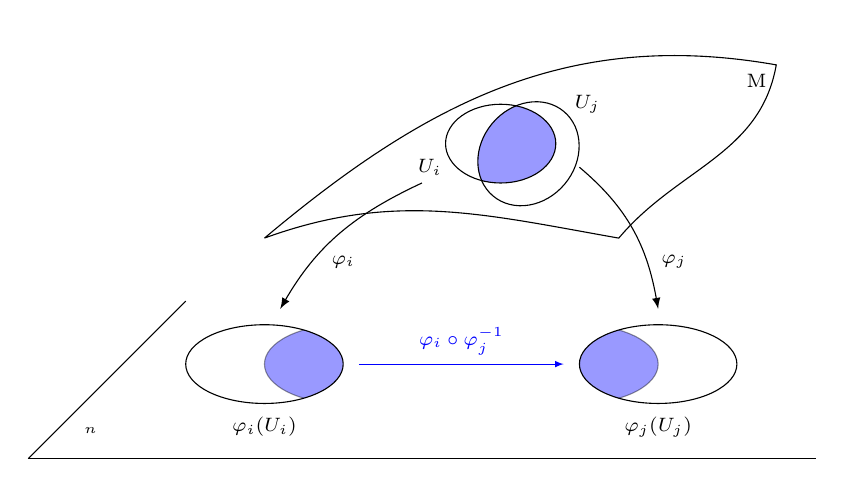
\begin{tikzpicture}[scale=1]
	\tikzstyle{every node}=[font=\scriptsize]
	\draw (0,0)  -- (10,0);
	\draw (0,0) -- (2,2);
	\node at (0.8,0.3) {$\mR^n$};
	
	\begin{scope}
	\clip (3,1.2) ellipse (1cm and 0.5cm);
	\draw [draw=black, fill=blue, opacity=0.4] (4,1.2) ellipse (1cm and 0.5cm);
	\end{scope}
	
	\begin{scope}
	\clip (8,1.2) ellipse (1cm and 0.5cm);
	\draw [draw=black, fill=blue, opacity=0.4] (7,1.2) ellipse (1cm and 0.5cm);
	\end{scope}
	
	\draw (3,1.2) ellipse (1cm and 0.5cm);
	\node at (3,0.4) {$\varphi_i(U_i) $};
	
	
	\draw [-latex] (5,3.5) to[out=-155,in=60] (3.2,1.9) node at (4,2.5) {$\varphi_i$};
	
	
	\draw (8,1.2) ellipse (1cm and 0.5cm);
	\node at (8,0.4) {$\varphi_j(U_j) $};
	
	\draw [-latex] (7,3.7) to[out=-40,in=100] (8,1.9) node at (8.2,2.5) {$\varphi_j$};
	
	
	\draw [ultra thin,-latex, color=blue] (4.2, 1.2) -- (6.8,1.2) node [pos=0.5,above] {$\varphi_i\circ\varphi_j^{-1}$};
	\draw (3,2.8) to[out=40,in=170] (9.5,5) node[below left] {$\mathrm{M}$} to[out=-100,in=50]  (7.5,2.8) to[out=170,in=20] (3,2.8);
	
	\node at (5.1,3.7) {$U_i$};
	\node at (7.1,4.5) {$U_j$};
	
	
	\begin{scope}
	\clip (6,4) ellipse (0.7cm and 0.5cm);
	\fill[blue, opacity=0.4, rotate around={-40:(6.2,4)}] (6.4,4) ellipse (0.6cm and 0.7cm);
	\end{scope}
	\draw [thin] (6,4) ellipse (0.7cm and 0.5cm);
	\draw [thin, rotate around={-40:(6.2,4)}] (6.4,4) ellipse (0.6cm and 0.7cm);
	
	\end{tikzpicture}
	\label{fig:atlas}
	\caption{A differentiable atlas on a manifold $\mM$.}
\end{figure}

\begin{definition}
	A \textbf{differentiable atlas} of a manifold $\mM$ is an atlas $\{U_i,\varphi_i\}_{i\in A}$ such that the functions
	$$\varphi_{ij}:=\textcolor{blue}{\varphi_i\circ\varphi_j^{-1}}:\varphi_j(U_i\cap U_j)\to\varphi_j(U_i\cap U_j),$$
	are differentiable (of class $C^\infty$) for any $i,j\in A$ such that $U_i\cap U_j\neq \emptyset$. Each $\varphi_{ij}$ is called \textbf{transition function}.
\end{definition}


	\noindent With this definition, each $\varphi_{ij}$ is a \textbf{diffeomorphism} because one can always interchange the indexes $i$ and $j$.\\



	\noindent We are only interested in \textbf{differentiable} (or \textbf{smooth}) \textbf{manifolds}, endowed with a maximal differentiable atlas. Here maximality of the atlas means that, if $\varphi$ is a chart of $\mM$ and $\{U_i,\varphi_i\}_{i\in A}$ is a differentiable atlas, then $\varphi$ belongs to $\{U_i,\varphi_i\}_{i\in A}$. We call a differentiable manifold with an atlas for which all chart transitions have positive Jacobian determinant an \textbf{orientable manifold}.
\begin{rem}
	For now on, the word \textbf{manifold} will always mean \textbf{differentiable manifold} and to indicate them it will be used the letters $\mM$ or $\mathrm{N}$.
\end{rem}


\begin{definition}[\textbf{Submanifold}]
	Let $n\leq m$. An $n$-dimensional \textbf{submanifold} $\mathrm{N}$ of $\mM$ is a nonempty subset $\mathrm{N}$ of $\mM$ such that, for every point $q\in\mathrm{N}$, there exists a local chart $\{U,\varphi\}$ of $\mM$ about $q$ such that
	$$\varphi(U\cap \mathrm{N})=\varphi(U)\cap(\mR^n\times\{0\})\subset\mR^m.$$ If $n=m-1$ we call $\mathrm{N}$ an \textbf{hypersurface} of $\mM$.
\end{definition}

\begin{example}
	If $\mM$ and $\mathrm{N}$ are manifolds, the Cartesian product $\mM\times\mathrm{N}$ is endowable with canonical structure of a manifold. If $\{U_i,\varphi_i\}_{i\in A}$ is an differentiable atlas for $\mM$ and $\{V_j,\psi_j\}_{j\in B}$ ia an atlas for $\mathrm{N}$, then $\big\{U_i\times V_j,(\varphi_i,\psi_j)\big\}_{(i,j)\in A\times B}$ is a differentiable atlas for $\mM\times\mathrm{N}$.
\end{example}

	\noindent As in the Euclidean case, one can introduce the notion of \textbf{differentiable} map between manifolds:
\begin{figure}[h]
	\centering
	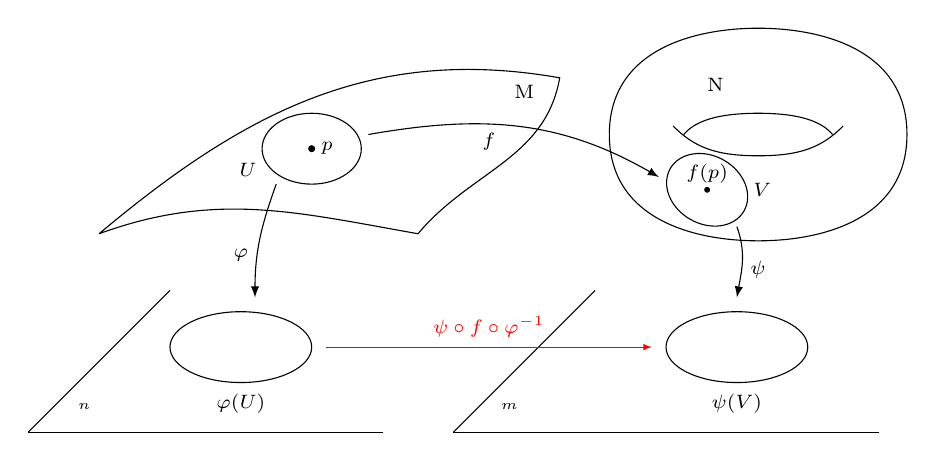
\begin{tikzpicture}[scale=0.9]
	\tikzstyle{every node}=[font=\scriptsize]
	\draw (0,0)  -- (5,0);
	\draw (0,0) -- (2,2);
	\node at (0.8,0.3) {$\mR^n$};
	\draw (6,0)  -- (12,0);
	\draw (6,0) -- (8,2);
	\node at (6.8,0.3) {$\mR^m$};
	
	
	
	
	\draw [thin] (3,1.2) ellipse (1cm and 0.5cm);
	\node at (3,0.4) {$\varphi(U) $};
	
	
	\draw [-latex] (3.5,3.5) to[out=-110,in=90] (3.2,1.9) node at (3,2.5) {$\varphi$};
	
	
	\draw [thin] (10,1.2) ellipse (1cm and 0.5cm);
	\node at (10,0.4) {$\psi(V) $};
	
	\draw [-latex] (10,2.9) to[out=-70,in=80] (10,1.9) node at (10.3,2.3) {$\psi$};
	
	\draw [-latex] (4.8,4.2) to[out=10,in=150] (8.9,3.6);
	\node at (6.5,4.1) {$f$};
	
	
	\draw [ultra thin,-latex, color=red] (4.2, 1.2) -- (8.8,1.2) node [pos=0.5,above] {$\psi\circ f\circ\varphi^{-1}$};
	
	
	\draw (1,2.8) to[out=40,in=170] (7.5,5) node at (7,4.8) {$\mathrm{M}$} to[out=-100,in=50]  (5.5,2.8) to[out=170,in=20] (1,2.8);
	
	\node at (3.1,3.7) {$U$};
	
	\draw [thin] (4,4) ellipse (0.7cm and 0.5cm);
	\fill [black] (4,4) circle (0.05cm) node [right] {$p$};
	
	\node at (9.7,4.9) {$\mathrm{N}$};
	
	\begin{scope}[shift={(10.3,4.2)},scale=0.6]
	
	
	
	\draw (-3.5,0) .. controls (-3.5,2) and (-1.5,2.5) .. (0,2.5);
	\draw[xscale=-1] (-3.5,0) .. controls (-3.5,2) and (-1.5,2.5) .. (0,2.5);
	\draw[rotate=180] (-3.5,0) .. controls (-3.5,2) and (-1.5,2.5) .. (0,2.5);
	\draw[yscale=-1] (-3.5,0) .. controls (-3.5,2) and (-1.5,2.5) .. (0,2.5);
	
	\draw (-2,.2) .. controls (-1.5,-0.3) and (-1,-0.5) .. (0,-.5) .. controls (1,-0.5) and (1.5,-0.3) .. (2,0.2);
	
	\draw (-1.75,0) .. controls (-1.5,0.3) and (-1,0.5) .. (0,.5) .. controls (1,0.5) and (1.5,0.3) .. (1.75,0);
	\draw [thin, rotate around={-30:(-1.2,-1.3)}] (-1.2,-1.3) ellipse (1cm and 0.8cm);
	\fill [black] (-1.2,-1.3) circle (0.07cm) node at (-1.2,-0.93) {$f(p)$};
	\node at (0.1,-1.3) {$V$};
	\end{scope}
	
	
	
	
	\end{tikzpicture}
	\label{fig:diffmap}
	\caption{The notion of differentiable map $f$ between manifolds $\mM$ and $\mathrm{N}$.}
\end{figure}

\begin{definition}
	A continuous map $f:\mM\to\mathrm{N}$ between two manifolds $\mM$ and $\mathrm{N}$ is \textbf{differentiable} at $p\in\mM$ if there exist local charts $\{U,\varphi\}$ and $\{V,\psi\}$ about $p$ in $\mM$ and about $f(p)$ in $\mathrm{N}$ respectively, such that $f(U)\subset V$ and
	$$ \textcolor{red}{\psi\circ f\circ \varphi^{-1}}:\varphi(U)\to\psi(V),$$
	is differentiable (of class $C^\infty$) at $\varphi(p)$. The function $f$ is said to be differentiable on $\mM$ if it is differentiable at every point of $\mM$.
\end{definition}

	\noindent The space of differentiable functions between two manifolds is denoted by $C^\infty(\mM,\mathrm{N})$, and if $\mathrm{N}=\mC$ simply by $C^\infty(\mM)$. If $\psi\circ f\circ \varphi^{-1}$ is of class $C^k$, we say $f\in C^k(\mM,\mathrm{N})$.\\

	\noindent We introduce the \textbf{tangent space} of a point of a manifold. %It may be thought as a local approximation of the $\mR^n$ structure that lies on the manifold.
It will be constructed using the derivatives of curves which pass through the point. A tangent vector at a point $p$ is thought of as the velocity of a curve passing through the point. We can therefore define a tangent vector as an equivalence class of curves passing through $p$ while being tangent to each other at $p$.
.\begin{definition}[\textbf{Tangent space}]
	Let $p\in\mM$ and let $I$ be an interval containing $0$. We indicate $\mathcal{C}_p=\{c\in C^\infty(I,\mM)|\ c(0)=p\}$ the set of differentiable curves passing through $p$.\\
	We consider the equivalence relation ($\sim$), according to which two curves $c_1,c_2\in\mathcal{C}_p$ are equivalent if there exists a local chart $\varphi$ about $p$ such that $(\varphi\circ c_1)'(0)=(\varphi\circ c_2)'(0)$.\\
	The \textbf{tangent space} of $\mM$ at $p$ is the set
	$\mT_p\mM:=\mathcal{C}_p/\sim.$
\end{definition}

\noindent We will refer at the equivalence class of curves with $\dot{c}$, as they are uniquely determined by the velocity $(\varphi\circ c)'(0)$ at which they pass through the point $p$.


	\noindent One can check that the definition of the equivalence relation does not depend on the choice of local chart. In fact, if $\{U,\varphi\}$ and $\{V,\psi\}$ are local charts at $p$,
\[ (\varphi\circ c)'(0)=(\varphi\circ\psi^{-1}\circ\psi\circ c)'(0)=D(\varphi\circ\psi^{-1})(\psi(p))\cdot(\psi\circ c)'(0),\]
where $D(\varphi\circ\psi^{-1})(\psi(p))$ stands for the Jacobian of the transition function calculated at $\psi(p)$. It holds that $(\varphi\circ c_1)'(0)$ and $(\varphi\circ c_2)'(0)$ coincide if and only if $(\psi\circ c_1)'(0)$ and $(\psi\circ c_2)'(0)$ coincide.\\

\begin{figure}[h]
	\centering
	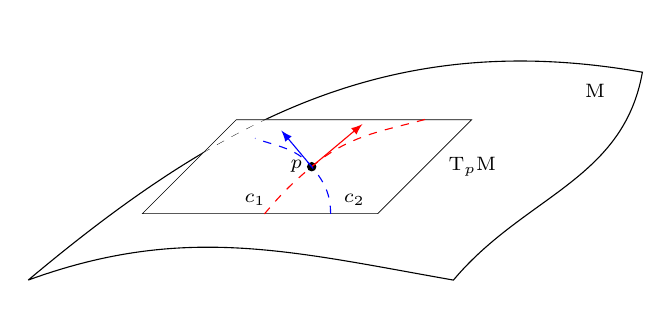
\begin{tikzpicture}[scale=1.2]
	\tikzstyle{every node}=[font=\scriptsize]
	
	\draw (1,2.8) to[out=40,in=170] (7.5,5) node at (7,4.8) {$\mathrm{M}$} to[out=-100,in=50]  (5.5,2.8) to[out=170,in=20] (1,2.8);
	
	\begin{scope}[shift={(0,0)},scale=1]
	\clip (2.2,3.5)-- (4.7,3.5) -- (5.7,4.5) -- (3.2,4.5) -- cycle;
	\draw [draw=black, fill=white] (2.2,3.5)-- (4.7,3.5) -- (5.7,4.5) -- (3.2,4.5) -- cycle;
	\draw [ultra thin, dashed] (1,2.8) to[out=40,in=170] (7.5,5) node at (7,4.8) {$\mathrm{M}$} to[out=-100,in=50]  (5.5,2.8) to[out=170,in=20] (1,2.8);
	
	\end{scope}
	\fill [black] (4,4) circle (0.05cm) node [left] {$p$};
	\node at (5.7,4) {$\mathrm{T}_p\mathrm{M}$};
	
	\draw [thin, dashed, color=red] (3.5,3.5) to[out=50,in=-140] (4,4) to[out=40,in=-165] (5.2,4.5);
	\begin{scope}[shift={(4,4)},scale=1]
	\draw [-latex, color=red] (0,0)-- (40:0.7cm);
	\end{scope}
	\node at (3.4,3.65) {$c_1$};
	
	\draw [thin, dashed, color=blue] (4.2,3.5) to[out=90,in=-50] (4,4) to[out=130,in=-20] (3.4,4.3);
	\begin{scope}[shift={(4,4)},scale=1]
	\draw [-latex, color=blue] (0,0)-- (130:0.5cm);
	\end{scope}
	\node at (4.45,3.65) {$c_2$};
	
	
	
	
	
	
	
	
	\end{tikzpicture}
	\label{fig:tangent}
	\caption{Tangent space $\mT_p\mM$ where $c_1\nsim c_2$.}
\end{figure}


	\noindent It can be proven that (for a fixed atlas $\varphi$ about $p$) the following map is a linear isomorphism between $\mT_p\mM$ and $\mR^n$:
$$\begin{aligned} \Theta_\varphi:\ \mT_p&\mM &\to\ &\mR^n,\\
							&\dot{c}&\mapsto \ & (\varphi\circ c)'(0).
   \end{aligned} $$
Hence we can think of $\mT_p\mM$ as being a copy of $\mR^n$ attached to the point $p$ on the manifold.\\
For reasons that we will make clear later, we denote the basis of $\mT_p\mM$ as
\[\left\{  \parz{ }{x^1}\Big|_p,\dots,\parz{ }{x^n}\Big|_p    \right\}.\]

	\noindent Collecting all tangent spaces, one builds the \textbf{tangent bundle} of a manifold $\mM$, defined as:
\[ \mT\mM=\bigsqcup_{p\in\mM} \mT_p\mM=\bigcup_{p\in\mM} \{p\}\times \mT_p\mM. \]



\begin{definition}
	Let $f:\mM\to\mathrm{N}$ be a differentiable map and let $p\in \mM$. The \textbf{differential} of $f$ at $p$ is the linear map
	\[\dd_p f:\mT_p\mM\to\mT_{f(p)}\mathrm{N},\quad \dot{c}\mapsto [f\circ c]\cong (f\circ c)'(0).   \]
	The \textbf{differential} of $f$ is the map $\dd f:\mT\mM\to\mT\mathrm{N}$ such that $\dd f|_{\mT_p\mM}=\dd_p f$.
\end{definition}


\begin{figure}[h]
	\centering
	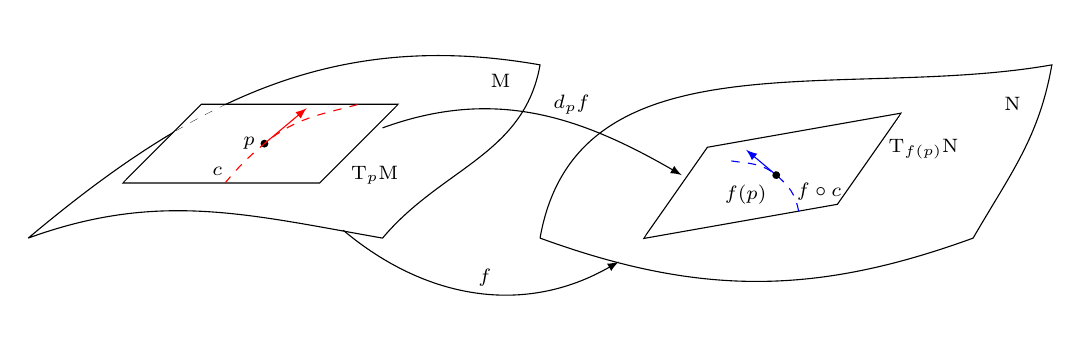
\begin{tikzpicture}[scale=1]
	\tikzstyle{every node}=[font=\scriptsize]
	
	\draw (1,2.8) to[out=40,in=170] (7.5,5) node at (7,4.8) {$\mathrm{M}$} to[out=-100,in=50]  (5.5,2.8) to[out=170,in=20] (1,2.8);
	
	\begin{scope}[shift={(0,0)},scale=1]
	\clip (2.15,3.45)-- (4.75,3.45) -- (5.75,4.55) -- (3.15,4.55) -- cycle;
	\draw [draw=black, fill=white] (2.2,3.5)-- (4.7,3.5) -- (5.7,4.5) -- (3.2,4.5) -- cycle;
	\draw [ultra thin, dashed] (1,2.8) to[out=40,in=170] (7.5,5) node at (7,4.8) {$\mathrm{M}$} to[out=-100,in=50]  (5.5,2.8) to[out=170,in=20] (1,2.8);
	
	\end{scope}
	
	\fill [black] (4,4) circle (0.05cm) node [left] {$p$};
	\node at (5.4,3.6) {$\mathrm{T}_p\mathrm{M}$};
	
	\draw [thin, dashed, color=red] (3.5,3.5) to[out=50,in=-140] (4,4) to[out=40,in=-165] (5.2,4.5);
	\begin{scope}[shift={(4,4)},scale=1]
	\draw [-latex, color=red] (0,0)-- (40:0.7cm);
	\end{scope}
	\node at (3.4,3.65) {$c$};
	
	\begin{scope}[shift={(6.5,0)},scale=1]
	\draw (1,2.8) to[out=80,in=190] (7.5,5) node at (7,4.5) {$\mathrm{N}$} to[out=-100,in=60]  (6.5,2.8) to[out=200,in=-20] (1,2.8);
	\end{scope}
	
	\begin{scope}[shift={(6.5,-0.4)},scale=1, rotate around={10:(4,4)}]
	\node at (5.9,4) {$\mathrm{T}_{f(p)}\mathrm{N}$};
	\clip (2.15,3.45)-- (4.75,3.45) -- (5.75,4.55) -- (3.15,4.55) -- cycle;
	\draw [draw=black, fill=white] (2.2,3.5)-- (4.7,3.5) -- (5.7,4.5) -- (3.2,4.5) -- cycle;
	%\draw [ultra thin, dashed] (1,2.8) to[out=40,in=170] (7.5,5) node at (7,4.8) {$\mathrm{M}$} to[out=-100,in=50]  (5.5,2.8) to[out=170,in=20] (1,2.8);
	
	\draw [thin, dashed, color=blue] (4.2,3.5) to[out=90,in=-50] (4,4) to[out=130,in=-20] (3.4,4.3);
	
	
	\begin{scope}[shift={(4,4)},scale=1]
	\draw [-latex, color=blue] (0,0)-- (130:0.5cm);
	\end{scope}
	\node at (4.5,3.7) {$f\circ c$};
	
	\fill [black] (4,4) circle (0.05cm) node [below left] {$f(p)$};
	
	\end{scope}
	
	\draw [-latex] (5,2.9) to[out=-40,in=-150] (8.5,2.5);
	\node at (6.8,2.3) {$f$};
	\draw [-latex] (5.5,4.2) to[out=20,in=150] (9.3,3.6);
	\node at (7.9,4.5) {$d_p f$};
	
	
	
	
	\end{tikzpicture}
	\label{fig:differential}
	\caption{A scheme of a differential map.}
	
\end{figure}

	\noindent Given $\mM$ and a chart $\{U, \varphi\}$ near $p$, fix $X=\dot{c}\in\mT_p\mM$. If we identify $\mT_p\mR\cong\mR$, we can interpret the differential $\dd_p f(X)$ of a function $f\in C^\infty(\mM)$ at a point $p$ as the \textbf{derivative} in the direction of $X$:
\[	\partial_X f(p):=\dd_p f(X).	\]
A functional which is linear and follows Leibniz rule, such as $\partial_X:C^\infty(\mM)\to\mR$, is called a \textbf{derivation}. The set of all derivations at $p$ is denoted as $\operatorname{Der}_p$ and it is a vector space. The map $X\in\mT_p\mM\mapsto\partial_X$ is an isomorphism between $\mT_p\mM$ and $\operatorname{Der}_p$.\\
Define:
\[	\parz{ }{x^i}\Big|_p:C^\infty(\mM)\to\mR,\quad f\mapsto\parz{f}{x^i}\Big|_p=\partial_X f(p),	\]
where $X=\dot{c}$ and $c(t)=\varphi^{-1}(\varphi(p)+te_i)$ ($e_i$ is the $i$-th canonical basis vector).\\
Note that, from the definition of the differential, it holds
\[ \partial_X f(p)=(f\circ c)'(0)=\parz{(f\circ \varphi^{-1})}{x^i}\Big|_{\varphi(p)},\]
which shows that the object we defined can be seen as a partial derivative in the usual sense.\\
It can be shown that the set of derivations $\{\parz{ }{x^1},\dots,\parz{ }{x^n}\}$ forms a basis for $\operatorname{Der}_p$ and, due to the isomorphism, for $\mT_p\mM$, $X$ can be expressed as
\[	X=X^i\parz{ }{x^i},	\]
where Einstein summation has been employed.\\
Observe that linearity entails that
\[	\partial_X f(p)=\dd_p f(X)=X^i\dd_p f\left(\parz{}{x^i}\Big|_p\right)=X^i\parz{f}{x^i}\Big|_p.		\]

\begin{figure}
	\centering
	\[
	\begin{tikzcd}[column sep=1.5em]
	& \mT_p\mM \arrow{dr}{\Theta_\varphi} \\
	\operatorname{Der}_p \arrow[<-]{ur}{X\mapsto \partial_X} && \mR^n
	\end{tikzcd}
	\]
	\caption{Isomorphism relations for the tangent space.}
\end{figure}






\begin{definition}
	Let $\mM$ be a manifold, we define a projection map $\pi:\mT\mM\to\mM$ such that $\pi(\mT_p\mM)=p$, and we call a \textbf{section} in the tangent bundle a map $s:\mM\to\mT\mM$ such that
	$\pi\circ s=\operatorname{id}_\mM.$
\end{definition}
	\noindent The dual space of the tangent space $\mT_p\mM$ is called the \textbf{cotangent space}, denoted with $\mT^*_p\mM$, which has a canonical basis denoted with $\{\dd x^1|_p,\dots,\dd x^n|_p\}$.\\
	The elements of such basis act on any element of the tangent space basis at $p$ as follows:
	\[	\dd x^i|_p\left(\parz{}{x^j}\Big|_p\right)=\delta_{ij}.		\]
	Similarly is defined the \textbf{cotangent bundle} $\mT^*\mM$ as the disjoint union of cotangent spaces.
	\begin{definition}
	Sections in the tangent bundle, denoted by $C^\infty(\mM,\mT\mM)$, are called \textbf{vector fields}, whereby sections in the cotangent bundle are called \textbf{$1$-forms}.
	\end{definition}

	Vector fields are locally expressed in terms of linear combinations of \[\left\{  \parz{ }{x^1},\dots,\parz{ }{x^n}    \right\}=:\left\{\partial_1,\dots,\partial_n\right\},\] where $\partial_i=\partial_i|_p$ at any point $p$, whereas $1$-forms are expressed as linear combinations of $$\{\dd x^1,\dots,\dd x^n\},$$
	where $\dd x^i$ is the $1$-form that acts at $p$ as $\dd x^i|_p$.




\begin{definition}
We define the derivative in the direction of $X$ as an operator $\partial_X:C^\infty(\mM)\to C^\infty(\mM)$ such that
	\[ \partial_X f=\dd f(X), \]
for any vector field $X\in C^\infty(\mM,\mT\mM)$.
\end{definition}
\noindent It follows immediately that Leibniz's rule holds: $\ds \partial_X (f\cdot g)=g\,\partial_Xf +f\,\partial_X g$, and again holds the useful formula
\[	\partial_X f=\dd f(X)=X^i\dd f(\partial_i)=X^i\parz{f}{x^i}.	\]

\begin{oss}
	Given two vector fields $X,Y\in C^\infty(\mM,\mT\mM)$, there is a unique vector field $[X,Y]\in C^\infty(\mM,\mT\mM)$ such that
	\[		\partial_{[X,Y]}f=\partial_X\partial_Y-\partial_Y\partial_X f \]
	for all $f\in C^\infty(\mM)$. The map $[\cdot,\cdot ]:C^\infty(\mM,\mT\mM)\times C^\infty(\mM,\mT\mM)\to C^\infty(\mM,\mT\mM)$ is called the \textbf{Lie bracket}, it is bilinear, skew-symmetric and satisfies the \emph{Jacobi identity}: for any $X,Y,Z\in C^\infty(\mM,\mT\mM)$ holds
	\[	\left[[X,Y],Z\right]+\left[[Y,Z],X\right]+\left[[Z,X],Y\right]=0.		\]
\end{oss}

\begin{definition}
	An \textbf{affine connection} or \textbf{covariant derivative} on a manifold $\mM$ is a bilinear map
	
	\[\begin{split}
	\nabla: C^\infty(\mM,\mT\mM)\times C^\infty(\mM,\mT\mM) & \rightarrow C^\infty(\mM,\mT\mM)\\
	(X,Y) & \mapsto \nabla_X Y\,,
	\end{split} \]
	such that for all smooth functions $f\in C^\infty(\mM)$ and all vector fields $X,Y\in C^\infty(\mM,\mT\mM)$:
	\begin{itemize}
		\item 	$\nabla_{fX}Y= f\nabla_X Y$, i.e., $\nabla$ is $C^\infty(\mM)-$linear in the first variable;
		\item $\nabla_Xf=\partial_X f$;
		\item $\nabla_X (fY) = Y\partial_X f+ f\nabla_X Y$, i.e., $\nabla$ satisfies the \emph{Leibniz rule} in the second variable.
	\end{itemize}
\label{defn:connection}
\end{definition}

\noindent The covariant derivative on the direction of the basis vector fields $\left\{\partial_1,\dots,\partial_n\right\}$ is indicated
\[	\nabla_{j}:=\nabla_{\partial_j}.	\]



\noindent We are now ready to introduce metric structures on manifolds.

\section{Lorentzian Manifolds}

In this section we will follow the approach delineated in [\citealp{pfaffle}] and in [\citealp[Ch. 1]{bar2}]. We start in the simple case of \textbf{Minkowski spacetime}.

\begin{definition}
	Let $V$ be an $n$-dimensional vector space. A \textbf{Lorentzian scalar product} is a nondegenerate symmetric bilinear form $\left\langle\cdot,\cdot\right\rangle$ with signature $(-+\dots +)$, i.e. such that one can find a basis $\{e_1,\dots, e_n\}$ such that
	\[	\left\langle e_1,e_1 \right\rangle=-1,\quad \left\langle e_i,e_j \right\rangle=\delta_{ij}\ \text{  if } i,j>1.	\]
	\end{definition}
\noindent The \textbf{Minkowski product} $\scalar{x}{y}_0$, defined by the formula
\[	\scalar{x}{y}_0=\eta_{ik}x^iy^k=-x_1\,y_1+x_2\,y_2+\cdots+x_n\,y_n,	\] with $\eta:=\operatorname{diag}(-1,1,\dots,1,1)$ is the simplest example of Lorentzian scalar product on $\mR^n$. The $n$-dimensional Minkowski space, denoted by $\mathbb{M}^n$ is simply $\mR^n$ equipped with Minkowski product.
	\begin{figure}[h]
		\centering
		\begin{tikzpicture}[scale=1.2]
		\tikzstyle{every node}=[font=\scriptsize]
		\draw [white,postaction={decorate,decoration={text along path,text align=center,text={|\scriptsize|lightlike}}}] (-1,1.3) to [bend right=60]  (1,1.3);
		
		\begin{scope}
		\clip (-2,2.5)-- (2,2.5) -- (-2,-2.5) -- (2,-2.5) -- cycle;
		\draw [dashed] (-1,1.2) to [bend right=60]  (1,1.2);
		\draw [dashed] (-1,-0.55) to [bend right=60]  (1,-0.55);
		\end{scope}
		
		
		
		\draw [white,postaction={decorate,decoration={text along path,text align=center,text={|\scriptsize|lightlike} }}] (-1,-0.5) to [bend right=50]  (1,-0.5);
		
		
		\draw [ultra thin, -latex] (-3,-2.5) -- (-3,2.5) node [below right]{$t$};
		\draw (2,2.5)-- (-2,-2.5);
		\draw (-2,2.5)-- (2,-2.5);
		\draw (0,2.5) ellipse (2 and 0.3);
		
		\draw (2,-2.5) arc[x radius=2, y radius=0.3, start angle=0, end angle=-180];
		\draw [dashed] (2,-2.5) arc[x radius=2, y radius=0.3, start angle=0, end angle=180];
		
		
		\fill [black] (0,0) circle (0.05cm) node at (-0.1,0) [left] {$0$};
		\node at (2,1.9) {$I_+(0)$};
		\node at (2,-1.9) {$I_-(0)$};
		\node at (0,1.8) {timelike};
		\node at (0,-1.8) {timelike};
		\node at (-1.5,0) {spacelike};
		\node at (1.5,0) {spacelike};
		
		
		
		\end{tikzpicture}
		
		\label{fig:mink}
		\caption{Minkowski time orientation.}
	\end{figure}
	
\begin{definition} We call the \textbf{negative squared length} of a vector $X\in V$
	\[\gamma(X)=-\norm{X}^2:=-\scalar{X}{X}. \]
	A vector $X\in V\setminus\{0\}$ is called
\begin{itemize}
	\item  \textbf{timelike} if $\gamma(X)>0$,
	\item \textbf{lightlike} if $\gamma(X)=0$,
	\item \textbf{spacelike} if $\gamma(X)<0$ or $X=0$,
	\item \textbf{causal} if it is either timelike or lightlike.
	\end{itemize}
\label{defn:gamma}
	\end{definition}
\noindent 	This definition will mostly be used for tangent vectors, in case $V$ is the tangent space of a Lorentzian manifold at a point.\\
	For $n\geq 2$ the set of timelike vectors $I(0)$ consists of two connected components. A \textbf{time orientation} is the choice of one of these two components, that we call $I_+(0)$.

	\begin{definition}	We call
	\begin{itemize}
		\item $J_+(0):=\overline{I_+(0)}$ (elements are called \textbf{future-directed}),
		\item $C_+(0):=\partial I_+(0)$ (upper \textbf{light cone}),
		\item $I_-(0):=-I_+(0)$, $J_-(0):=-J_+(0)$ (elements are called \textbf{past-directed}),
		\item $C_-(0):=-C_+(0)$ (lower \textbf{light cone}).
	\end{itemize}
	\end{definition}

	


\begin{definition}
	A \textbf{metric} $g$ on a manifold $\mM$ is the assignment of a scalar product at each tangent space $$g:\mT_p\mM\times\mT_p\mM\to\mR$$ which depends smoothly on the base point $p$. We call it a \textbf{Riemannian metric} if the scalar product is pointwise positive definite, and a \textbf{Lorentzian metric} if it is a Lorentzian scalar product.\\
	A pair $(\mM,g)$, where $\mM$ is a manifold and $g$ is a Lorentzian (Riemannian) metric is called a \textbf{Lorentzian (Riemannian) manifold}.
\end{definition}
\noindent The request of smooth dependence on $p$ may be specified as follows: given any chart $\{U,\varphi=(x^1,\dots,x^n)\}$ about $p$, the functions $g_{ij}:\varphi(U)\to\mR$ defined by $g_{ij}=g(\parz{ }{x^i},\parz{ }{x^j})$, for any $i,j=1,\dots,n$ should be differentiable. With respect to these coordinates one writes
\[ g=\sum_{i,j} g_{ij}\,\dd x_i\otimes \dd x_j\equiv\sum_{i,j}g_{ij}\,\dd x_i\, \dd x_j. \]

The scalar product of two tangent vectors $v,w\in\mT_p\mM$, with coordinate chart $\varphi=(x^1,\dots x^n)$, such that $v=v^i\parz{ }{x^i}$, $w=w^j\parz{ }{x^j}$ is
\[ \langle v,w\rangle=g_{ij}(\varphi(p))v^iw^j.   \]
When the choice of the chart is clear we will often write, with abuse of notation $g_{ij}(p):=g_{ij}(\varphi(p))$. We will indicate $(g^{ij})_{i,j=1,\dots, n}=(g_{ij})^{-1}$.\\

\noindent The \textbf{negative squared length} of a tangent vector $X$ at $p\in\mM$ generalizes naturally as follows:
\begin{equation}
	\gamma(X)=-\langle X,X\rangle.
	\label{eq:gamma}
\end{equation}

\noindent From now on $\mM$ will always indicate a \textbf{Lorentzian manifold}.

\begin{definition}
		A vector field $X\in C^\infty (\mM,\mT\mM)$ is called timelike, spacelike, lightlike or causal, if $X (p)$ is timelike, spacelike, lightlike or causal, respectively, at every point $p\in\mM$.\\
		
		\noindent A differentiable curve $c : I\to\mM$ is called timelike, lightlike,
		spacelike, causal, future-directed or past-directed if $\dot{c}(t)\in\mT_{c(t)}\mM$ is, for all $t\in I$, timelike, lightlike, spacelike, causal,
		future-directed or past-directed, respectively.\\
		
		\noindent A Lorentzian manifold $\mM$ is called \textbf{time-oriented} if there exists a nowhere vanishing timelike vector field on $\mM$. If a manifold is time-oriented, we refer to it as \textbf{spacetime}.
\end{definition}


\begin{figure}[h]
\centering
	\begin{subfigure}{.5\textwidth}

	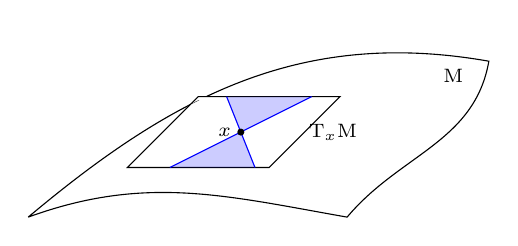
\begin{tikzpicture}[scale=0.9]
	\tikzstyle{every node}=[font=\scriptsize]
	
	\draw (1,2.8) to[out=40,in=170] (7.5,5) node at (7,4.8) {$\mathrm{M}$} to[out=-100,in=50]  (5.5,2.8) to[out=170,in=20] (1,2.8);
	
	\begin{scope}[shift={(0,0)},scale=1]
	\clip (2.2,3.4)-- (4.7,3.4) -- (5.7,4.6) -- (3.2,4.6) -- cycle;
	\draw [draw=black, thin, fill=white] (2.4,3.5)-- (4.4,3.5) -- (5.4,4.5) -- (3.4,4.5) -- cycle;
	\draw [ultra thin, dashed] (1,2.8) to[out=40,in=170] (7.5,5) node at (7,4.8) {$\mathrm{M}$} to[out=-100,in=50]  (5.5,2.8) to[out=170,in=20] (1,2.8);
	
	\draw [thin, color=blue, fill=blue, fill opacity=0.2] (3,3.5) -- (4,4) -- (4.2,3.5) ;
	
	\draw [thin, color=blue, fill=blue, fill opacity=0.2] (3.8,4.5) -- (4,4) -- (5,4.5);
	
	%\draw [thin, color=blue, fill=blue, fill opacity=0.2] (3,3.5) -- (5,4.5)-- (3.8,4.5) -- (4.2,3.5) -- (3.8,4.5);
	
	
	\end{scope}
	\fill [black] (4,4) circle (0.05cm) node [left] {$x$};
	\node at (5.3,4) {$\mathrm{T}_x\mathrm{M}$};
	
	\end{tikzpicture}
	\caption{A time-oriented tangent space.}
	\end{subfigure}

	\begin{subfigure}{.5\textwidth}

			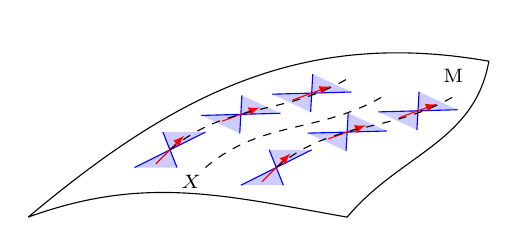
\begin{tikzpicture}[scale=0.9]
		\tikzstyle{every node}=[font=\scriptsize]
		
		\draw (1,2.8) to[out=40,in=170] (7.5,5) node at (7,4.8) {$\mathrm{M}$} to[out=-100,in=50]  (5.5,2.8) to[out=170,in=20] (1,2.8);
		
	
	\begin{scope}[shift={(-0.5,0.25)},scale=1]
	
	
	\begin{scope}[shift={(1.5,1.5)},scale=0.5]
	\clip (2.2,3.4)-- (4.7,3.4) -- (5.7,4.6) -- (3.2,4.6) -- cycle;
	\draw [thin, color=blue, fill=blue, fill opacity=0.2] (3,3.5) -- (4,4) -- (4.2,3.5) ;
	\draw [thin, color=blue, fill=blue, fill opacity=0.2] (3.8,4.5) -- (4,4) -- (5,4.5);
	\begin{scope}[shift={(4,4)},scale=1]
	\draw [-latex, color=red] (-0.4,-0.4)-- (0.4,0.4);
	\end{scope}
	
	\end{scope}
	
	\begin{scope}[shift={(2.5,2)},scale=0.5, rotate around={-25:(4,4)}]
	\clip (2.2,3.4)-- (4.7,3.4) -- (5.7,4.6) -- (3.2,4.6) -- cycle;
	\draw [thin, color=blue, fill=blue, fill opacity=0.2] (3,3.5) -- (4,4) -- (4.2,3.5) ;
	\draw [thin, color=blue, fill=blue, fill opacity=0.2] (3.8,4.5) -- (4,4) -- (5,4.5);
	\begin{scope}[shift={(4,4)},scale=1]
	\draw [-latex, color=red] (-0.4,-0.4)-- (0.4,0.4);
	\end{scope}
	\end{scope}
	
	\begin{scope}[shift={(3.5,2.3)},scale=0.5, rotate around={-25:(4,4)}]
	\clip (2.2,3.4)-- (4.7,3.4) -- (5.7,4.6) -- (3.2,4.6) -- cycle;
	\draw [thin, color=blue, fill=blue, fill opacity=0.2] (3,3.5) -- (4,4) -- (4.2,3.5) ;
	\draw [thin, color=blue, fill=blue, fill opacity=0.2] (3.8,4.5) -- (4,4) -- (5,4.5);
	\begin{scope}[shift={(4,4)},scale=1]
	\draw [-latex, color=red] (-0.4,-0.4)-- (0.4,0.4);
	\end{scope}
	\end{scope}
	
	\draw [ dashed, color=black] (3.5,3.5) to[out=40,in=-150] (6,4.5);
	\end{scope}
	
	\begin{scope}[shift={(1,0)},scale=1]
	
	
	\begin{scope}[shift={(1.5,1.5)},scale=0.5]
	\clip (2.2,3.4)-- (4.7,3.4) -- (5.7,4.6) -- (3.2,4.6) -- cycle;
	\draw [thin, color=blue, fill=blue, fill opacity=0.2] (3,3.5) -- (4,4) -- (4.2,3.5) ;
	\draw [thin, color=blue, fill=blue, fill opacity=0.2] (3.8,4.5) -- (4,4) -- (5,4.5);
	\begin{scope}[shift={(4,4)},scale=1]
	\draw [-latex, color=red] (-0.4,-0.4)-- (0.4,0.4);
	\end{scope}
	
	\end{scope}
	
	\begin{scope}[shift={(2.5,2)},scale=0.5, rotate around={-25:(4,4)}]
	\clip (2.2,3.4)-- (4.7,3.4) -- (5.7,4.6) -- (3.2,4.6) -- cycle;
	\draw [thin, color=blue, fill=blue, fill opacity=0.2] (3,3.5) -- (4,4) -- (4.2,3.5) ;
	\draw [thin, color=blue, fill=blue, fill opacity=0.2] (3.8,4.5) -- (4,4) -- (5,4.5);
	\begin{scope}[shift={(4,4)},scale=1]
	\draw [-latex, color=red] (-0.4,-0.4)-- (0.4,0.4);
	\end{scope}
	\end{scope}
	
	\begin{scope}[shift={(3.5,2.3)},scale=0.5, rotate around={-25:(4,4)}]
	\clip (2.2,3.4)-- (4.7,3.4) -- (5.7,4.6) -- (3.2,4.6) -- cycle;
	\draw [thin, color=blue, fill=blue, fill opacity=0.2] (3,3.5) -- (4,4) -- (4.2,3.5) ;
	\draw [thin, color=blue, fill=blue, fill opacity=0.2] (3.8,4.5) -- (4,4) -- (5,4.5);
	\begin{scope}[shift={(4,4)},scale=1]
	\draw [-latex, color=red] (-0.4,-0.4)-- (0.4,0.4);
	\end{scope}
	\end{scope}
	
	\draw [ dashed, color=black] (3.5,3.5) to[out=40,in=-150] (6,4.5);
	\end{scope}
	\draw [ dashed, color=black] (3.5,3.5) to[out=40,in=-150] (6,4.5);
	\node at (3.3,3.3) {$X$};
		
		\end{tikzpicture}
	\caption{A time-oriented manifold together with field lines of a timelike vector field $X$.}
	\end{subfigure}
	\label{fig:timemanif}
	\caption{Time orientations.}
\end{figure}

The \textbf{causality relations} on $\mM$ are defined as follows. Let $p,q\in\mM$,
\begin{itemize}
	\item $p\ll q$ iff there exists a future-directed timelike curve from $p$ to $q$,
	\item $p< q$ iff there is a future-directed causal curve from $p$ to $q$,
	\item $p\le q$ iff $p<q$ or $p=q$.
\end{itemize}
\noindent The causality relation "$<$" is a strict weak ordering and the relation "$\le$" makes the manifold a partially ordered set.\\

\begin{definition}
	The \textbf{chronological future} of a point $x\in\mM$ is the set $I_+^M(x)$ of points that can be reached by future-directed \textsl{timelike} curves, i.e.
	\[		I_+^M(x)=\{y\in\mM\ |\ x<y\}.	\]
	The \textbf{causal future} $J_+^M(x)$ of a point $x\in\mM$ is the set of points that can be reached by future-directed \textsl{causal} curves from $x$, i.e.,
	\[	J_+^M(x)=\{y\in\mM\ |\ x\le y\}.	\]
	Given a subset $A\subset \mM$ the \textbf{chronological future} and the \textbf{causal future} of $A$ are respectively
	\[	I_+^M(A)=\bigcup_{x\in A}I_+^M(x),\qquad J_+^M(A)=\bigcup_{x\in A}J_+^M(x).	\]
	In a similar way, one defines the \textbf{chronological} and \textbf{causal pasts} of a point $x$ of a subset $A \subset \mM$ by replacing \textsl{future-directed curves} with \textsl{past directed curves}. They are denoted by $I_-^M (x), I_-^M (A), J_-^M (x)$, and $J_-^M (A)$, respectively. We will also use the notation $J^M (A) := J_-^M (A) \cup J_+^M (A)$.
\end{definition}
\noindent Any subset $\Omega$ of a spacetime $\mM$ is a spacetime itself, if one restricts the metric to $\Omega$. So $I_{\pm}^{\Omega}(x)$ and $J_{\pm}^{\Omega}(x)$ are well defined.
\begin{definition}
	A subset $\Omega\subset\mM$ of a spacetime is called \textbf{causally compatible} if for any point $x\in\Omega$ holds
	\[	J_{\pm}^{\Omega}(x)=J_{\pm}^{\mM}(x)\cap\Omega,		\]
	where it can be noted that the inclusion "$\subset$" always holds.
\end{definition}

\noindent The condition we defined means that taken two points in $\Omega$ that can be joined by a causal curve in $\mM$, there also exists a causal curve connecting them inside $\Omega$.\\

\begin{figure}[h]
	\centering\begin{tikzpicture}
	\tikzstyle{every node}=[font=\scriptsize]
	\draw [black] plot [smooth cycle] coordinates { (0,0) (1,1) (3,0) (1.5,-1)};
	\node at (1.5,0) {$A$};
	\begin{scope}[shift={(2.7,-0.42)},scale=1]
	\draw [color=red] (0,0) -- (45:3cm);
	\end{scope}
	
	\begin{scope}[shift={(2.9,0.13)},scale=1]
	\draw [color=blue] (0,0) -- (-45:2.5cm);
	\end{scope}
	
	\begin{scope}[shift={(0.25,-0.33)},scale=1]
	\draw [color=red] (0,0) -- (135:3cm);
	\end{scope}
	
	
	\begin{scope}[shift={(0.3,0.58)},scale=1]
	\draw [color=blue] (0,0) -- (-135:3cm);
	\end{scope}
	
	\node at (1.5,1.7) {$J_+^M(A)$};
	\node at (1.5,-1.7) {$J_-^M(A)$};
	%\draw [ultra thin, -latex] (-2.5,-2.5) -- (-2.5,2.5) node [below right]{$t$};
	\end{tikzpicture}
	\label{fig:causalfuturepast}
	\caption{Causal future $J_+^M$ and causal past $J_-^M$ of a subset $A\subset\mM$. }
\end{figure}


\noindent We now can introduce the concept of \textbf{geodesics} and \textbf{exponential map}.

\begin{definition}
	Let $c : [a,b]\to \mM$ be a curve on a Lorentzian manifold $\mM$. The
	length $L\dot{c}$ is defined by (with Einstein summation convention )
	\[ L\dot{c}=\int_{a}^{b} \sqrt{|g(\dot{c}(t),\dot{c}(t))|}\,d t=\int_{a}^{b} \sqrt{\left|g_{ik}(c(t)) \deri{x^i}{t}\deri{x^k}{t}\right|}\,d t,\]
	where $x^i(t):=(\varphi\circ c)^i(t)$ are the coordinates of the point $c(t)$ in a chart $\varphi$.\\
	Given $p,q\in\mM$, if $p\leq q$ we define the \textbf{time-separation} between $p$ and $q$ as
	\[\tau(p,q)=\sup\{L[c]\ |\ c \text{ is a future directed causal curve from }p\text{ to } q\}, \]
	and $0$ otherwise.\\
	A \textbf{geodesic} between two points $p,q\in\mM$ such that $p\leq q$, if it exists, is a curve $c$ such that $L[c]=\tau(p,q)$, i.e. the curve of maximum time-separation.
\end{definition}
\noindent The request on the geodesics implies that (in variational sense) $\delta L\dot{c}=0$. It can be demonstrated that the stationary problem for the functional $L\dot{c}$ is equivalent to $\delta E\dot{c}=0$ for the functional, called \textbf{energy}, defined by
\[		E\dot{c}=\frac{1}{2}\int_{a}^{b} {|g(\dot{c}(t),\dot{c}(t))|}\,d t.	\]
Since the Euler-Lagrange equations for a functional $I[c]=\int_{a}^{b} f(t,c(t),\dot{c}(t))\, dt$ read
\[		\deri{ }{t}\left(\parz{f}{\dot{x}^i}\right)-\parz{f}{x^i}=0,	\]
being $c=(x^1,\dots,x^n)$, then, in our case, setting $f(t,c,\dot{c})=g(\dot{c},\dot{c})$:
\[  \frac{\dd^2 x^i}{\dd t^2}-\Gamma_{jk}^i\deri{x^j}{t}\deri{x^k}{t}=0.	\]
Here $\Gamma_{jk}^i\in C^\infty (U\subset\mM)$ are the \textbf{Christoffel symbols}, defined in the chart $\varphi=(\xi^1,\dots,\xi^n)$ as
\[	\Gamma_{jk}^i=\frac12 \sum_l g^{il} \left(
\frac{\partial g_{lj}}{\partial \xi^k} 
+\frac{\partial g_{lk}}{\partial \xi^j}
-\frac{\partial g_{jk}}{\partial \xi^l}
\right).	\]

\begin{definition}
	A connection $\nabla$ on a manifold $\mM$ with a metric $g$ is said to be a \textbf{metric connection} if for all $X,Y,Z\in C^\infty (\mM,\mT\mM)$ holds the following \emph{Leibniz rule}:
	\[		\partial_X\,g(Y,Z)=g(\nabla_X Y, Z)+g(Y,\nabla_X Z).	\]
	The unique metric connection which is also torsion-free, i.e.,
	\[		T:=\nabla_X Y-\nabla_Y X-[X,Y]=0,	\]
	is called the \textbf{Levi-Civita connection}. 
\end{definition}

\noindent Another way to define \textbf{geodesics} is to say a geodesic between two points $p,q$ on a manifold $\mM$ with the Levi-Civita connection $\nabla$ is the curve $c$ which links $p$ and $q$ such that parallel transport along it preserves the tangent vector to the curve, i.e.
\begin{equation}
	\nabla_{\dot{c}(t)}\dot{c}(t)=0\quad \text{for all } t\in [a,b].
	\label{eq:LCgeodesic}
\end{equation}
More precisely, in order to define the covariant derivative of $\displaystyle \dot{c}$ it is necessary first to extend $\displaystyle \dot{c}$ to a smooth vector field in an open set containing the image of the curve, but it can be shown that the derivative is independent of the choice of the extension.\\

\begin{oss}
	We can express the Christoffel symbols in terms of the Levi-Civita connection:
	\begin{equation}
			\nabla_{j}\partial_k=\Gamma_{jk}^i \partial_i
			\label{eq:LCchrist}
	\end{equation}
in a local chart $\varphi=(x^1,\dots,x^n)$.
\end{oss}

\begin{prop}
	Let $\nabla$ be a connection over a manifold $\mM$ and $X,Y\in C^\infty(\mM,\mT\mM)$ be vector fields. It holds
	\[	\nabla_X Y=\left(X^j\partial_jY^k+X^jY^i\Gamma_{ij}^k\right)\partial_k,		\]
	in particular
	\[	(\nabla_j Y)^i=\partial_jY^i+Y^i\Gamma_{ij}^k.		\]
\end{prop}
\Proof From Definition \ref{defn:connection} holds:
\[	\nabla_X Y=\nabla_{X^je_j}Y^i e_i=X^j\partial_j Y^i e_i=X^jY^i\nabla_j e_i+X^j e_i\partial_j Y^i=		\]
\[	=X^jY^i\Gamma_{ij}^k e_k+(X^j\partial_jY^k) e_k	.	\]


\begin{prop}
	Let us consider $p\in\mM$ and a tangent vector $\xi\in \mT_p\mM$. Then there exists $\epsilon>0$ and precisely one geodesic $$c_\xi:[0,\epsilon]\to\mM,$$ such that $c_\xi(0)=p$ and $\dot c_\xi(0)=\xi$.
\end{prop}

\begin{definition}
	In the conditions of the proposition above, if we put
	\[		\mathcal{D}_p=\{	\xi\in\mT_p\mM\ |\ c_\xi \text{ is defined on } [0,1]	\}\subset \mT_p\mM,	\]
	the \textbf{exponential map} at point $p$ is defined as $\exp_p:\mathcal{D}_p\to\mM$ such that $\exp_p(\xi)=c_\xi(1)$.\\
	The local coordinates defined by the chart $\{U:=\exp_p(\mathcal{D}_p),\exp_p^{-1} \}$ are called \textbf{normal coordinates} centered at $p$.
\end{definition}

\begin{figure}[h]
	\centering
		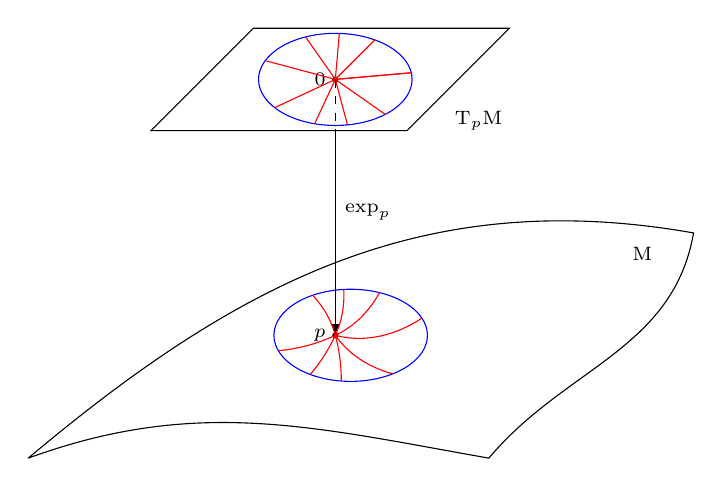
\begin{tikzpicture}[scale=1.3]
	\tikzstyle{every node}=[font=\scriptsize]
	
	\draw (1,2.8) to[out=40,in=170] (7.5,5) node at (7,4.8) {$\mathrm{M}$} to[out=-100,in=50]  (5.5,2.8) to[out=170,in=20] (1,2.8);
	
	\begin{scope}[shift={(0,2.5)},scale=1]
		\node at (5.4,3.6) {$\mathrm{T}_p\mathrm{M}$};
	%\clip (2.2,3.6)-- (4.7,3.5) -- (5.7,4.5) -- (3.2,4.5) -- cycle;
	\draw [draw=black, fill=white] (2.2,3.5)-- (4.7,3.5) -- (5.7,4.5) -- (3.2,4.5) -- cycle;
	\fill [black] (4,4) circle (0.03cm) node [left] {$0$};
	\draw [draw=blue, rotate around={0:(4,4)}] (4,4) ellipse (0.75cm and 0.45cm);
	
	\end{scope}
	
	\begin{scope}[shift={(4,6.5)},scale=1]
	\clip (0,0) ellipse (0.75cm and 0.45cm);
	\foreach \x in {0,...,9}
	\draw [thin, color=red] (0,0)-- ({5+40*\x}:2cm);
	\end{scope}
	
	
	\draw [ dashed] (4,6.5) -- (4,6);
	\draw [ -latex] (4,6) -- (4,4) node [pos=0.4, right] {$\exp_p$};
	
	
	\begin{scope}[shift={(0,0)},scale=1]
	%\clip (2.2,3.6)-- (4.7,3.5) -- (5.7,4.5) -- (3.2,4.5) -- cycle;
	\fill [black] (4,4) circle (0.03cm) node [left] {$p$};
	\draw [draw=blue, rotate around={0:(4,4)}] (4.15,4) ellipse (0.75cm and 0.45cm);
	
	\end{scope}
	
	\begin{scope}[shift={(4,4)},scale=1]
	\clip (0.15,0) ellipse (0.75cm and 0.45cm);
	\foreach \x in {0,...,4}
	\draw [thin, color=red] (0,0) to [bend right=60] ({5+40*\x}:2cm);
	\foreach \x in {4,...,6}
	\draw [thin, color=red] (0,0) to [bend left=40] ({5+40*\x}:2cm);
	\end{scope}
	
	
	\end{tikzpicture}
	\label{fig:exp}
	\caption{The exponential maps from the tangent space to the manifold.}
\end{figure}

\begin{prop}
	Given normal coordinates centered at $p\in\mM$, it holds
	\[	g_{ij}(p):=g_{ij}(\exp_p(0))=\eta_{ij},\] \[ \Gamma_{jk}^i=0,	\]
	for all indexes $i,j,k$.
\end{prop}

\noindent We are now ready to talk about \textbf{geodesically starshaped} sets.


\begin{definition}
	An open subset $\Omega\subset\mM$ is called \textbf{geodesically starshaped} with respect to a point $p\in\mM$ if there exists an open subset $\Omega'\subset\mT_p\mM$, starshaped with respect to 0, such that the exponential map
	\[	\exp_p|_{\Omega'}:\Omega'\to\Omega,		\]
	is a diffeomorphism. If $\Omega$ is geodesically starshaped with respect to all of its points, one calls it \textbf{convex}.
\end{definition}

\begin{prop}
	Under the conditions of the last definition, let $\Omega\subset\mM$ be geodesically starshaped with respect to point $p\in\mM$. Then one has
	\[	I_{\pm}^\Omega(p)=\exp_p(I_{\pm}(0)\cap\Omega'),		\]
	\[	J_{\pm}^\Omega(p)=\exp_p(J_{\pm}(0)\cap\Omega').		\]
\end{prop}

\noindent We continue our preparations with another function that we are going to need in Chapter (3).

\begin{definition}
	Let $\Omega\subset\mM$ be open and geodesically starshaped with respect to $x\in\Omega$. We define 
	\[	\Gamma_x:=\gamma\circ\exp_x^{-1}:\Omega\to\mR,		\]
	where $\gamma:\mT_x\mM\to\mR$ is defined in equation (\ref{eq:gamma}).
	\label{defn:Gamma}
\end{definition}


\subsection{Causality and Global Hyperbolicity}



Now we introduce causal domains, because they will appear in the theory of wave equations. The local construction of fundamental solutions is always possible on causal domains, provided they are small enough.


\begin{definition}
	A domain $\Omega\subset\mM$ is called \textbf{causal} if its closure $\overline{\Omega}$ is contained in a convex domain $\Omega'$ and for any $p,q\in\overline{\Omega}$ $J_{+}^{\Omega'}(p)\cap J_{-}^{\Omega'}(q)$ is compact and contained in $\overline{\Omega}$.\\
	A subset $A\subset\mM$ is called \textbf{past-compact} (respectively \textbf{future-compact}) if, for all $p\in\mM$, $A\cap J_-^{\mM}(p)$ (respectively $A\cap J_+^{\mM}(p)$) is compact.
	\label{defn:pastcompact}
\end{definition}

\begin{figure}[h]
	\centering
	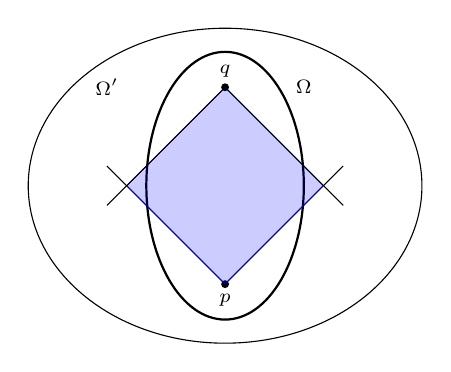
\begin{tikzpicture}
	\draw[thin] (0,0) ellipse (2.5 and 2);
	\draw[thick] (0,0) ellipse (1 and 1.7);
	\fill [black] (0,1.25) circle (0.05cm) node [above] {$q$};
	\fill [black] (0,-1.25) circle (0.05cm) node [below] {$p$};
	\begin{scope}[shift={(0,-1.25)},scale=1]
	\draw (0,0) -- (1.5,1.5);
	\draw (0,0) -- (-1.5,1.5);
	\clip (0,0) -- (1.25,1.25) -- (0,2.5) -- (-1.25,1.25) -- cycle;
	\draw [thin, color=blue, fill=blue, fill opacity=0.2] (0,0) -- (1.25,1.25) -- (0,2.5) -- (-1.25,1.25) -- cycle;
	\end{scope}
	\begin{scope}[shift={(0,1.25)},scale=1]
	\draw (0,0) -- (1.5,-1.5);
	\draw (0,0) -- (-1.5,-1.5);
	\end{scope}
	\node at (1,1.25) {$\Omega$};
	\node at (-1.5,1.25) {$\Omega'$};
	\end{tikzpicture}
	\caption{Convex, but non causal, domain}
\end{figure}

\noindent We can notice that, if we look at compact spacetimes, something physically unsound occurs: 

\begin{prop}
	If a spacetime $\mM$ is compact, there exists a closed timelike curve in $\mM$.
	\label{prop:paradoxes}
\end{prop}
\noindent In a few words, there are manifolds, such as compact spacetimes, where there are timelike loops that can produce science fictional paradoxes. To avoid such unphysical and unrealistic things we require suitable causality conditions:
\begin{definition}
	A spacetime satisfies the \textbf{causality condition} if it does not contain any closed causal curve. A spacetime $\mM$ satisfies the \textbf{strong causality condition} if there are no almost closed causal curves, i.e. if for any $p\in\mM$ there exists a neighborhood $U$ of $p$ such that there exists no timelike curve that passes through $U$ more than once.
\end{definition}
\noindent It is clear that the strong causality condition implies the causality condition.
\begin{figure}
	\centering
	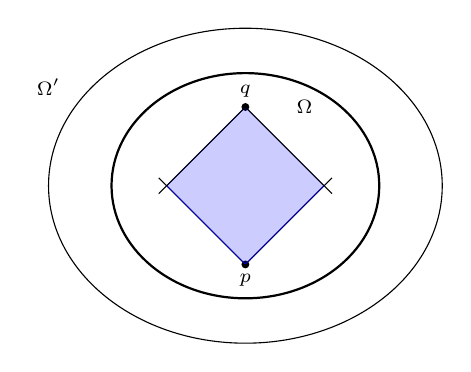
\begin{tikzpicture}
	\draw[thin] (0,0) ellipse (2.5 and 2);
	\draw[thick] (0,0) ellipse (1.7 and 1.43);
	\fill [black] (0,1) circle (0.05cm) node [above] {$q$};
	\fill [black] (0,-1) circle (0.05cm) node [below] {$p$};
	\begin{scope}[shift={(0,-1)},scale=1]
	\draw (0,0) -- (1.1,1.1);
	\draw (0,0) -- (-1.1,1.1);
	\clip (0,0) -- (1,1) -- (0,2) -- (-1,1) -- cycle;
	\draw [thin, color=blue, fill=blue, fill opacity=0.2] (0,0) -- (1,1) -- (0,2) -- (-1,1) -- cycle;
	\end{scope}
	\begin{scope}[shift={(0,1)},scale=1]
	\draw (0,0) -- (1.1,-1.1);
	\draw (0,0) -- (-1.1,-1.1);
	\end{scope}
	\node at (0.75,1) {$\Omega$};
	\node at (-2.5,1.25) {$\Omega'$};
	\end{tikzpicture}
	\caption{Causal domain}
\end{figure}
\begin{definition}
	A spacetime $\mM$ that satisfies the strong causality condition and such that for all $p,q\in\mM$ $J_+^{\mM}(p)\cap J_-^{\mM}(q)$ is compact is called \textbf{globally hyperbolic}.
	\label{defn:globalhyp}
\end{definition}

\noindent It can be demonstrated that in globally hyperbolic manifolds for any $p\in\mM$ and any compact set $K\subset\mM$ the sets $J_{\pm}^{\mM}(p)$ and $J_{\pm}^{\mM}(K)$ are closed.

\begin{definition}
	A subset $S$ of a connected time-oriented Lorentzian manifold $\mM$ is a \textbf{Cauchy hypersurface} if each inextensible timelike curve (i.e. no reparametrisation of the curve can be continuously extended) in $\mM$ meets $S$ at exactly one point.
	\label{defn:Cauchyhyper}
\end{definition}


\begin{figure}
	\begin{subfigure}{.5\textwidth}
	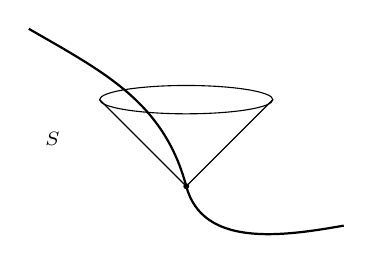
\begin{tikzpicture}
	\draw[thick] (-2,2) to[out=-30,in=105] (0,0) to[out=-75,in=190] (2,-0.5);
	\draw (0,0) -- (1.1,1.1);
	\draw (0,0) -- (-1.1,1.1);
	\draw (0,1.1) ellipse (1.1 and 0.18);
	\draw[fill=black] (0,0) circle (0.03cm);
	\node at (-1.7,0.6) {$S$};
	\end{tikzpicture}
	\caption{A non-Cauchy hypersurface}
\end{subfigure}
\begin{subfigure}{.5\textwidth}
	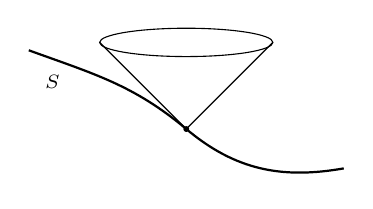
\begin{tikzpicture}
	\draw[thick] (-2,1) to[out=-20,in=140] (0,0) to[out=-40,in=190] (2,-0.5);
	\draw (0,0) -- (1.1,1.1);
	\draw (0,0) -- (-1.1,1.1);
	\draw (0,1.1) ellipse (1.1 and 0.18);
	\draw[fill=black] (0,0) circle (0.03cm);
	\node at (-1.7,0.6) {$S$};
	\end{tikzpicture}
	\caption{A Cauchy hypersurface}
\end{subfigure}
\caption{Hypersurfaces.}
\end{figure}


\noindent In other words, no point of a Cauchy hypersurface is in the light cone of another point of the surface.
\begin{theorem}
	Let $\mM$ be a connected time-oriented Lorentzian manifold. Then the following are equivalent:
	\begin{itemize}
		\item $\mM$ is globally hyperbolic.
		\item There exists a Cauchy hypersurface in $\mM$.
		\item $\mM$ is isometric to $\mR\times S$ with metric $g=-\beta\dd t^2+b_t$, where $\beta$ is a smooth positive function, $b_t$ is a Riemannian metric on $S$ depending smoothly on $t$ and each $\{t\}\times S$ is a smooth Cauchy hypersurface in $\mM$.
	\end{itemize}
	In such case there exists a smooth function $h:\mM\to\mR$ whose gradient is past-directed timelike at every point and all of whose level sets are Cauchy hypersurfaces.
	\label{th:Bernal}
\end{theorem}
\noindent We briefly give some examples of globally hyperbolic spacetimes.
\begin{example}
	The Minkowski spacetime $\mathbb{M}^n$ is globally hyperbolic. Every
	spacelike hyperplane is a Cauchy hypersurface. We have $\mathbb{M}^n=\mR\times S$ with $S = \mR^{n-1}$ , endowed	with the time-independent Euclidean metric.\\
	
\noindent	Let $S$ be a Riemannian manifold with time independent metric $b_t$ and $I\subset\mR$ an interval. Let $f: I\to\mR$
	be a smooth positive function. The manifold $\mM=I \times S$ with the metric $g = -\dd t^2 + f^2(t)\, b_t$, called \textbf{cosmological spacetime},
	is globally hyperbolic if and only if $S$ is a complete space, see [\citealp[Lem A.5.14]{bar1}]. This applies in particular if $S$ is compact.\\
	
	\noindent The interior and exterior \textbf{Schwartzschild spacetimes}, that represent non-rotating black holes of mass $m>0$ are globally hyperbolic.\\
	Denoting $S^2$ the $2$-dimensional sphere embedded in $\mR^3$, we set
	\[	\mM_{\text{ext}}:=\mR\times(2m,+\infty)	\times S^2,	\] 
	
	\[	\mM_{\text{int}}:=\mR\times(0,2m)	\times S^2.	\] 
	The metric is given by
	\[	g=-h(r)\dd t^2+\frac{1}{h(r)}\dd r^2	+r^2\,g_{S^2},	\]
	where $h(r)=1-\frac{2m}{r}$, while $g_{S^2}=r^2\,\dd\theta^2+r^2\sin^2\theta\dd\varphi^2$ is the polar coordinates metric on the sphere. For the exterior Schwartzschild spacetime we have $\mM_{\text{ext}}=\mR\times S$ with $S=(2m,+\infty)\times S^2$, $\beta=h$ and $b_t=\frac{1}{h(r)}\dd r^2	+r^2\,g_{S^2}$.
	\label{ex:spacetimes}
\end{example}




\section{Operators and integration on manifolds}
\label{sec:operators}
We call $C_0^\infty(\mM)$ the set of $C^\infty$ functions on a manifold with compact support. The integral map\footnote{see [\citealp[Ch. A.3]{bar1}]} is defined as the unique map
\[	\int_{\mM}\cdot\ \dd\mu:C_0^\infty(\mM)\to \mC,	\]
such that it is linear and for any local chart $\{U,\varphi\}$ and for any $f\in C_0^\infty(U)$ holds
\[	\int_{\mM}f\,\dd\mu=\int_{\varphi(U)}(f\circ\varphi^{-1})(x)\,\mu_x\,\dd x,		\]
where we define \begin{equation}
	\mu_x:=|\det g(x)|^{1/2}.
	\label{eq:mu}
\end{equation}

\noindent In this section we introduce the \textbf{generalized d'Alembert} operators, whose general form in local coordinates is given by
\begin{equation}
	P=-g^{ij}(x)\frac{\partial^2}{\partial x^i\partial x^j}+a_j(x)\parz{}{x^j}+b(x).
%	\label{eq:generalizedAlembert}
\end{equation}
The d'Alembert wave operator $\Box$ is defined for smooth functions $f$ as
\[	\Box f=-\operatorname{div}\grad f,	\]
where $\grad f$ is a vector field defined by the requirement that the formula $$\scalar{\grad f}{X}=\partial_X f$$ holds for any vector field $X$. At the same time $\operatorname{div}$ is defined as follows
\begin{definition}
	The \textbf{divergence} of a vector field $Z=Z^i\partial_i$ is defined as
	\[	\operatorname{div}Z=\sum_{j}(\nabla_j Z)_j=\partial_jZ^j+\Gamma_{ij}^iZ^j.	\]
\end{definition}

\begin{prop}
	The following formula holds:
	\begin{equation}
		\operatorname{div}Z=\mu_x^{-1}\parz{}{x^j}\left(\mu_xZ^j\right),
		\label{eq:divergence}
	\end{equation}
		
\noindent 	and the definition of divergence is consistent with that of integral.
\end{prop}
\Proof Let $h\in C_0^\infty(\mM)$; using integration by parts
\[	\int_{\mM} h\cdot\operatorname{div}(Z)\dd\mu=-\int_\mM Z^j \partial_j h\,\dd\mu = -\int_\mM Z^j \partial_j h\, \mu_x\,\dd x.	\]
Now integrating by parts again in the chart it holds:
\[	-\int_\mM \partial_j h\  Z^j \mu_x\, \dd x= \int_\mM h\ \partial_j (\mu_x\, Z^j)\, \dd x = \int_\mM h\ \mu_x^{-1}\partial_j(\mu_x\ Z^j)\, \dd\mu.		\]
Since this is true for any function $h$, the formula is proven.\endproof\\

\noindent From the definition of gradient one can show
\[g_{ij}(\grad f)^iX^j=\partial_X f=X^j\parz{f}{x^j},\quad \grad f=g^{ij}\parz{f}{x^i}\partial_j.\]
Hence it holds
\[	\Box f=-\mu_x^{-1}\parz{}{x^j}\left(\mu_x\, g^{ij}\parz{f}{x^i}\right).	\]
In Minkowski spacetime, where $g=\eta$,
\[	\Box f=-\parz{}{x^j}\left(\eta^{jj}\parz{f}{x^j}\right)=\frac{\partial^2f}{\partial t^2}-\sum_{i=1}^{n-1}\frac{\partial^2f}{\partial x_i^2}=-\partial^i\partial_if.		\]


